\documentclass[10pt,xetex]{beamer} %[compress, blue]
\mode<presentation>


\setbeamercolor{frametitle}{fg=lightred,bg=darkred}
\setbeamercolor{title}{fg=lightred,bg=darkred}

\usepackage[russian,english]{babel}

\usepackage{multirow}
\usepackage{fontspec}
\usepackage{xunicode}
\usepackage{xltxtra}
\usepackage{wasysym}
\usepackage{url}

\newcommand{\compresslist}{
	\setlength{\itemsep}{1pt}
	\setlength{\parskip}{0pt}
	\setlength{\parsep}{0pt}
}


\newfontfeature{IPA}{+mgrk}
\defaultfontfeatures{Mapping=tex-text} %PunctuationSpace=3,Scale=MatchLowercase,,Numbers=Lining}
\setmainfont[]{Nimbus Sans L}
\setsansfont[]{Nimbus Sans L}
\setmonofont[]{FreeMono}
\newfontfamily\qipa[IPA,Scale=MatchLowercase]{FreeSerif}

% Chuvash colours are 203,0,0 and 255,254,0
\definecolor{darkred}{RGB}{153,0,0}
\definecolor{lightred}{RGB}{226,200,200}
\definecolor{yellow}{RGB}{226,226,50}


\usetheme{Warsaw}

\usecolortheme[named=darkred]{structure}


\newfontfamily\cyrtext[Scale=MatchLowercase]{Nimbus Sans L}
\useoutertheme[subsection=false]{smoothbars}
%\setbeamertemplate{footline}[page number]{} % header empty
% \setbeamercolor{footer}{fg=blue,bg=lightred}
%\setbeamercolor{footline}{fg=white,bg=lightred} 
%    \setbeamercolor{page number in head/foot}{use=headline,fg=headline.fg,bg=frametitle.fg}
\setbeamertemplate{footline}[page number]{} % header empty

\setbeamertemplate{headline}[text line]{} % header empty

\setbeamertemplate{navigation symbols}{}

\newcommand{\atag}[1]{{\scriptsize{\texttt{#1}}}}
\newcommand{\itemise}{\itemize}

%\date{20th May 2012}
\date{}
\title{A prototype machine translation system for Tatar and Bashkir \\
              based on free/open-source components}

%\author{Francis M. Tyers \and Jonathan North Washington \\ 
%       U.A \and I.U \\
%Ilnar Salimzyanov \and Rustam Battalov}
%
%\author{{\bf Francis M. Tyers}\\ {\tt \href{mailto:ftyers@dlsi.ua.es}{ftyers@dlsi.ua.es}}\\Dept. de Lleng. i Sist. Inform.,\\Universitat d'Alacant \and
%{\bf Jonathan North Washington}\\ {\tt \href{mailto:jonwashi@indiana.edu}{jonwashi@indiana.edu}}\\Department of Linguistics,\\Indiana University\\
%{\bf Ilnar Salimzyanov} \and
%{\bf Rustam Battalov} 
%}
\usepackage{natbib}
\begin{document}

\begin{frame}
        \titlepage
\centering
\vspace{-4em}
\begin{tabular}{cc}
 {\bf Francis M. Tyers} & {\bf Jonathan North Washington} \\
 Grup Transducens & Depts. Linguistics \&\\
 Dept. Lleng. i Sist. Inform. & Central Eurasian Studies \\
 Universitat d'Alacant & Indiana University \\
 {\tt \href{mailto:ftyers@dlsi.ua.es}{ftyers@dlsi.ua.es}} & {\tt \href{mailto:jonwashi@indiana.edu}{jonwashi@indiana.edu}} \\ 
 ~ & ~ \\
 {\bf Ilnar Salimzyanov} & {\bf Rustam Batalov} \\
 Department of Russian Philology & Department of Economics \\ 
 Kazan Federal University & Bashkir State University \\
 {\tt \href{mailto:ilnar.salimzyan@gmail.com}{ilnar.salimzyan@gmail.com}} & {\tt \href{mailto:taqmaq@mail.ru}{taqmaq@mail.ru}} \\
 ~ & ~ \\
\end{tabular}

\end{frame}

%%%%%%%%%%%%%%%%%%%%%%%%%%%%%%%%%%%%%%%%%%%%%%%%%%%%%%%%%%%%%%%%%%%%%%%%%%%%%%%
\begin{frame}
  \frametitle{Introduction}
  
  \begin{onlyenv}<1>
    \begin{block}{Layout of the talk}
    
      \begin{itemize}
        \item Introduction
        \item Description of architecture and development process
        \item Evaluation
        \item Discussion and future work
      \end{itemize}
    
    \end{block}
  \end{onlyenv}
  
  \begin{onlyenv}<2>
    \begin{block}{Why make a Tatar $\leftrightarrow$ Bashkir MT system?}
    
      \begin{itemize}
        \item There are quite a few examples of MT systems made with Apertium
        \begin{itemize}
          \item but no working examples between ``morphologically complex'' languages
        \end{itemize}
    
        \item Course in Šupaškar (Čeboksary), January 2012
        \begin{itemize}
          \item Nearly all the languages of Russia are ``morphologically complex'', but
              we had no example system to present.
        \end{itemize} 
    
        \item The idea was to create a pedagogical example
        \begin{itemize}
          \item A simple demonstration system 
          \item that nonetheless showed all modules working
        \end{itemize}
     
        \item We chose Tatar and Bashkir because,
        \begin{itemize}
          \item Native speakers available to help out
          \item Good results could be accomplished with little work
        \end{itemize}
      \end{itemize}
    \end{block}
  \end{onlyenv}
  
\end{frame}

\begin{frame}
  \frametitle{Tatar and Bashkir} % Map
  \framesubtitle{Geography}
	%\begin{centering}
		\vspace{0.2em}
		\noindent\hspace{-2.75em}\includegraphics[width=1.175\textwidth]{middlevolga19001500.jpg}
	%\end{centering}
\end{frame}
\begin{frame}
	\frametitle{Tatar and Bashkir}
	\framesubtitle{Demographics}
    
    \begin{block}{Tatar}
      
      \begin{itemize}
        \item spoken by $>$ 6.5m people \citep{lewis2009}
		  \item coofficial with Russian in Tatarstan
		  \item minority language even in Tatarstan
		  \item high rate of bilingualism with Russian
      \end{itemize}
      
    \end{block}
      
    \begin{block}{Bashkir}
      
      \begin{itemize}
        \item spoken by $>$ 1.3m people \citep{lewis2009}
		  \item coofficial with Russian in Bashqortostan
		  \item minority language even in Bashqortostan
		  \item high rate of bilingualism with Russian
		  \item classified as ``vulnerable'' by UNESCO
      \end{itemize}
    
    \end{block}
\end{frame}
\begin{frame}
	\frametitle{Tatar and Bashkir}
	\framesubtitle{Comparison}
 
  \begin{onlyenv}<1>
	 \begin{block}{The similarities}
	 	\begin{itemize}\compresslist
			\item very close relatives: same branch of Kypchak group of Turkic
			\item share many innovations
			\item high level of mutual intelligibility when spoken
			\item large percentage of the lexicon are similar
		\end{itemize}
	\end{block}

	\begin{block}{The differences}
		\begin{itemize}\compresslist
			\item Bashkir has quite a few phonological innovations not found Tatar
			\begin{itemize}
				\item handful of extra historical changes
				\item rounding harmony
				\item desonorisation of high-sonority suffix-initial consonants\\cf.\ \citet{washington10}
			\end{itemize}
			\item a number of morphological differences
			\begin{itemize}
				\item e.g., different volitional participles
			\end{itemize}
			\item many inherent similarities are obscured:
			\begin{itemize}
				\item phonological and morphological differences
				\item different orthographical systems
			\end{itemize}
		\end{itemize}
	\end{block}
  \end{onlyenv}
  \begin{onlyenv}<2>
	\begin{block}{A sentence}
		\begin{itemize}
			\item[{\small {\tt tat}}] Һава бүген бик әйбәт, җылы гына.  \\
			{\qipa [hɑwɑ bɵɣɘn bijk æjbæt, ʑələ ʁənɑ]}
			\item[{\small {\tt bak}}] Һауа бөгөн бик әйбәт, йылы ғына. \\
			{\qipa [hɑwɑ bɵɣɵn bik æjbæt, jələ ʁənɑ]}
		\end{itemize}
	\end{block}

		\begin{block}{Volitional participles}
			\begin{itemize}
				\item[{\small {\tt tat}}] Барасым килә. `\textit{I want to go}'
				\item[{\small {\tt bak}}] Барғым килә. `\textit{I want to go}'\\
				Бараһым килә.
			\end{itemize}	
		\end{block}

		\begin{block}{Phonology: desonorisation}
			\begin{itemize}
				\item[{\small {\tt tat}}] башны `\textit{head-ACC}'
				\item[{\small {\tt bak}}] башты `\textit{head-ACC}'
			\end{itemize}	
			cf.\ \citet{washington10}
		\end{block}

  \end{onlyenv}
  \begin{onlyenv}<3>
  
    %FIXME: Check IPA with native speakers
	(transcriptions are approximate)
	\begin{block}{Tatar and Bashkir}
		\begin{itemize}
			\item[{\small {\tt tat}}] Һава бүген бик әйбәт, җылы гына.  \\
			{\qipa [hɑwɑ bɵɣɘn bijk æjbæt, ʑələ ʁənɑ]}
			\item[{\small {\tt bak}}] Һауа бөгөн бик әйбәт, йылы ғына. \\
			{\qipa [hɑwɑ bɵɣɵn bik æjbæt, jələ ʁənɑ]}
		\end{itemize}
	\end{block}

	\begin{block}{Comparison with other Turkic languages}
		\begin{itemize}
			\item[{\small {\tt tur}}] Hava bugün çok güzel, yeterince sıcak. \\
			{\qipa [hɑvɑ buɣyn ʧok gyzæl, jɛtʰɛrɪnʤɛ sɯʤɑkʰ]}
			\item[{\small {\tt chv}}] Ҫанталӑк паян питӗ хитре, самай ӑшӑ. \\
			{\qipa [ɕanˈtalək pɑˈjɑn ˈpitɘ xitˈre, saˈmaj ˈɔʂə]}
			\item[{\small {\tt kaz}}] Ауа райы бүгін әбден жақсы, жылы. \\
			{\qipa [ɑwɑ ɾɑjə bʉɣɘn æbdi̯ɘn ʐɑχsə, ʐələ]}
			\item[{\small {\tt kir}}] Аба ырайы бүгүн аябай жакшы, жылуу. \\
			{\qipa [ɑβɑ ɾɑjɯ βyɣyn ɑjɑβɑj ʥɑqʃɯ, ʥɯluː]}
		\end{itemize}
	\end{block}
  
  \end{onlyenv}
  
\end{frame}

\begin{frame}
  \frametitle{Apertium}

\begin{center}
  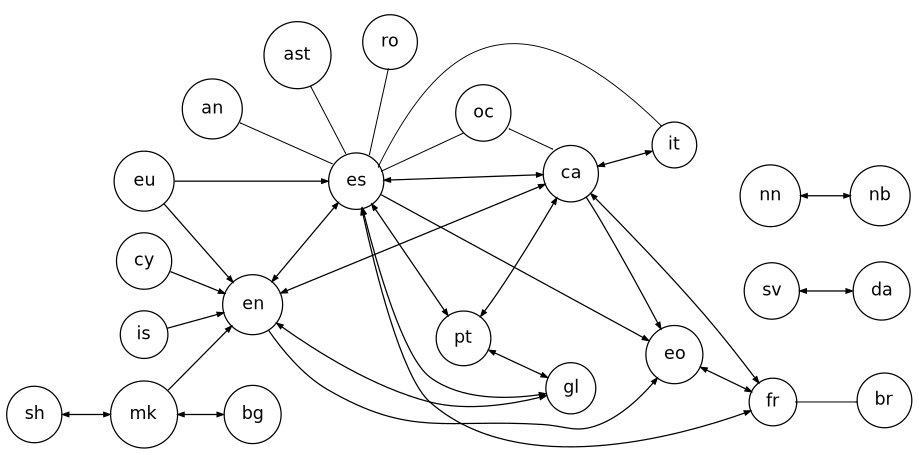
\includegraphics[width=0.82\textwidth]{apertiumlangs.pdf}%FIXED: svg->pdf is ugly
\end{center}

\begin{block}{Overview}
  
  \begin{itemize}
    \item Free/open-source software (GPL licence)
    \begin{itemize}
      \item Not only the programs, but the data too!
    \end{itemize}
    \item Fairly mature data for over 30 language pairs
    \item ... but so far no mature data for Turkic languages!
  \end{itemize}
  
\end{block}


\end{frame}

%%%%%%%%%%%%%%%%%%%%%%%%%%%%%%%%%%%%%%%%%%%%%%%%%%%%%%%%%%%%%%%%%%%%%%%%%%%%%%%
\begin{frame}
  \frametitle{Architecture}

\includegraphics[width=\textwidth]{architecture-ap.pdf} 
\vspace{1em}
\hrule
\vspace{1em}
\includegraphics[width=\textwidth]{architecture-ko.pdf} 
\begin{flushright}
{\tiny Machine translation between Turkic languages (Tantuğ et al., 2007)}
\end{flushright}

\end{frame}

\begin{frame}
  \frametitle{Tools}

  \begin{block}{Helsinki Finite-State Toolkit (HFST)}
    \begin{itemize}
      \item Free/open-source implementation of the Xerox 
         finite-state formalisms {\small {\tt lexc}}/{\small {\tt twol}}
      \item Used for morphological analysis and generation
    \end{itemize}
		\begin{center}
		{\small \url{http://hfst.sf.net/}}
		\end{center}
  \end{block}
  
  \begin{block}{VISL Constraint Grammar}
    \begin{itemize}
      \item Rule-based morphological disambiguation
    \end{itemize}
		\begin{center}
		{\small \url{http://beta.visl.sdu.dk/constraint\_grammar.html}}
		\end{center}

  \end{block}
  
  \begin{block}{Apertium}
    \begin{itemize}
      \item Lexical and structural transfer
      \item ``Platform'': Build system, ancilliary tools, etc.
    \end{itemize}
		\begin{center}
		{\small \url{http://www.apertium.org/} }
		\end{center}

  \end{block}
  
\end{frame}


\begin{frame}[fragile]


\begin{onlyenv}<1->
\fontsize{9pt}{11.2}\selectfont
  \begin{tabular*}{\textwidth}{l}
  %\hline
  %{\bf Stage} & {\bf Representation} \\
  \hline
  \hline
   Һава бүген бик әйбәт, җылы гына. \\ 
  \hline
  \end{tabular*}
\end{onlyenv}

\begin{onlyenv}<2->
\fontsize{9pt}{11.2}\selectfont
  \begin{tabular*}{\textwidth}{l}
  {\bf Morphological analysis} \\
  \hline
   \^{}Һава/һава\atag{<n>}\atag{<attr>}/һава\atag{<n>}\atag{<nom>\$} \^{}бүген/бүген\atag{<adv>\$}  \\
                \^{}бик/бик\atag{<adv>}/бик\atag{<n>}\atag{<attr>}/бик\atag{<n>}\atag{<nom>\$} \\ 
                \^{}әйбәт/әйбәт\atag{<adj>}/әйбәт\atag{<adj>}\atag{<subst>}\atag{<nom>\$}\^{},/,\atag{<cm>\$} \\ 
                \^{}җылы/җылы\atag{<n>}\atag{<attr>}/җылы\atag{<n>}\atag{<nom>}/җылы\atag{<adj>}/җылы\atag{<adj>}\atag{<subst>}\atag{<nom>\$} \\
                \^{}гына/гына\atag{<postadv>\$}\^{}./.\atag{<sent>\$} \\
  \hline
  \end{tabular*}
\end{onlyenv}

\begin{onlyenv}<3->
\fontsize{9pt}{11.2}\selectfont
  \begin{tabular*}{\textwidth}{l}
  {\bf Morphological disambiguation} \\
  \hline
   \^{}Һава\atag{<n>}\atag{<nom>\$} \^{}бүген\atag{<adv>\$} \^{}бик\atag{<adv>\$} \^{}әйбәт\atag{<adj>\$}\^{},\atag{<cm>\$} \\ 
                \^{}җылы\atag{<adj>\$} \^{}гына\atag{<postadv>\$}\^{}.\atag{<sent>\$}\\
  \hline
  \end{tabular*}
\end{onlyenv}

\begin{onlyenv}<4->
\fontsize{9pt}{11.2}\selectfont
  \begin{tabular*}{\textwidth}{l}
  {\bf Lexical transfer and selection} \\
  \hline
   \^{}Һава\atag{<n>}\atag{<nom>}/Һауа\atag{<n>}\atag{<nom>\$} \^{}бүген\atag{<adv>}/бөгөн\atag{<adv>\$} \^{}бик\atag{<adv>}/бик\atag{<adv>\$} \\
                \^{}әйбәт\atag{<adj>}/әйбәт\atag{<adj>\$}\^{},\atag{<cm>}/,\atag{<cm>\$} \^{}җылы\atag{<adj>}/йылы\atag{<adj>\$} \\ 
                \^{}гына\atag{<postadv>}/ғына\atag{<postadv>\$}\^{}.\atag{<sent>}/.\atag{<sent>\$}\\
  \hline
  \end{tabular*}
\end{onlyenv}

\begin{onlyenv}<5->
\fontsize{9pt}{11.2}\selectfont
  \begin{tabular*}{\textwidth}{l}
  {\bf Structural transfer} \\
  \hline
   \^{}Һауа\atag{<n>}\atag{<nom>\$} \^{}бөгөн\atag{<adv>\$} \^{}бик\atag{<adv>\$} \^{}әйбәт\atag{<adj>\$}\^{},\atag{<cm>\$} \\ 
                \^{}йылы\atag{<adj>\$} \^{}ғына\atag{<postadv>\$}\^{}.\atag{<sent>\$}\\
  \hline
  \end{tabular*}
\end{onlyenv}

\begin{onlyenv}<6->
\fontsize{9pt}{11.2}\selectfont
  \begin{tabular*}{\textwidth}{l}
  {\bf Morphological generation}\\
  \hline
   Һауа бөгөн бик әйбәт, йылы ғына. \\
  \hline
  \end{tabular*}
\end{onlyenv}

\end{frame}

%%%%%%%%%%%%%%%%%%%%%%%%%%%%%%%%%%%%%%%%%%%%%%%%%%%%%%%%%%%%%%%%%%%%%%%%%%%%%%%
\begin{frame}
  \frametitle{Development process}

  \begin{itemize} % FIXME: check this
    \item Stems in both Tatar and Bashkir are added to an online spreadsheet
    \begin{itemize}
      \item Added according to frequency in the RNC. % downsides: Well, I think that translation from a third X language is always a bit dangerous,
                                                     % because it leads to duplication of stems. Another thing is (if the language we are translating
                                                     % from is distant from other two), one has to be careful and not forget to check POS tags.
                                                     % Me and Rustam forgot it often /or was it before me :)?/ and we got lot's of miscategorizations
                                                     % when Russian adj. was translated with a n.attr (and the <adj> remained). It wasn't that bad initially,
                                                     % but after introducing n.attr tag they clearly became mistakes.
                                                     %
                                                     % The best way seems to be to collect a corpus (somehow, even a small one) for one of the languages,
                                                     % and translate wordforms from it by their frequency. And it turned out to be faster that way, becuase
                                                     % sometimes you don't have to change anything at all, if wordform is actually a lemma. Just copy and paste it.
                                                     % 
                                                     % For some semiclosed categories (like country names) Wikipedia might be useful. E.g., look at the
                                                     % category with all contry names and get them from there. (Let's see if I can use this for kaz-tat) /I.S./                 

      \item At the same time as translations, POS categories are added, and some
        relevant subcategorisations (transitivity, Tatar infinitive)
    \end{itemize}
    \item Scripts are used to automate the process of converting the spreadsheet
       to bilingual ({\small {\tt .dix}}) and monolingual ({\small {\tt .lexc}}) formats.
    \item At the same time, the morphotactics and phonology are written
       according to available grammatical descriptions
    
  \end{itemize}
\end{frame}

\begin{frame}[fragile]
  \frametitle{Development speed}
  \framesubtitle{Coverage and number of stems / time}

\begin{onlyenv}<1>
\begin{center}

%\vspace{1pt}
%\noindent\hspace{-4em}
\begin{tabular}{cc}
\includegraphics[angle=270,width=0.5\textwidth]{hist-tt-dec.ps} &  \includegraphics[angle=270,width=0.5\textwidth]{hist-ba-dec.ps} \\
Tatar & Bashkir \\
\end{tabular}

\end{center}
\end{onlyenv}

\begin{onlyenv}<2>
\begin{center}
\begin{tabular}{cc}
\includegraphics[angle=270,width=0.5\textwidth]{hist-tt-mar.ps} &  \includegraphics[angle=270,width=0.5\textwidth]{hist-ba-mar.ps} \\
Tatar & Bashkir \\
\end{tabular}
\end{center}
\end{onlyenv}


\end{frame}

%%%%%%%%%%%%%%%%%%%%%%%%%%%%%%%%%%%%%%%%%%%%%%%%%%%%%%%%%%%%%%%%%%%%%%%%%%%%%%%
\begin{frame}
  \frametitle{Evaluation}

\begin{block}{Rules and lexica}
  \begin{center}
    \begin{tabular}{lr}
    \hline
     {\bf Corpus}                        & {\bf Entries}\\
    \hline
     Bilingual dictionary                & 2,685     \\
     Disambiguation ({\small {\tt tt}} and {\small {\tt ba}}) & 6   \\
     Transfer ({\small {\tt tt$\rightarrow$ba}}) & 3 \\
     Transfer ({\small {\tt ba$\rightarrow$tt}}) & 3 \\
    \hline
    \end{tabular}
  \end{center}  

\end{block}

\begin{block}{Coverage}

\begin{center}
  \begin{tabular}{lrr}
  \hline
   {\bf Corpus}             & {\bf Tokens}    & {\bf Coverage}\\
  \hline
   Tatar New Testament (NT) & 163,603   & 72.04\% \\
   Tatar Wikipedia          & 37,123    & 70.19\% \\
  \hline
   Bashkir Wikipedia        & 12,267    & 65.99\% \\
  \hline
  \end{tabular}

\end{center}
\end{block}

\begin{block}{Error rate}
\begin{center}
  % NOTE: The performance without MT is:
  %        tt->ba: 56,59% 
  %        ba->tt: 56,41% 
  % simple 'transliteration' (e.g. ҙ ҡ ғ ҫ → з к г с; ч җ ъ → с й ø):
  %        ba->tt: 46.47%
  %        tt->ba: 54,98%
  \begin{tabular}{ccrrr} 
  \hline
   {\bf Corpus}           & {\bf Direction}   & {\bf Tokens}  & {\bf Unknown} & {\bf WER}  \\
  \hline
   \multirow{2}{*}{story} & {\small {\tt tt$\rightarrow$ba}} & 311     & 2  & 6.73\% \\
                          & {\small {\tt ba$\rightarrow$tt}} & 312     & 0  & 6.43\%  \\
  \hline
  \end{tabular}
\end{center}
\end{block}

\end{frame}

\begin{frame}
  \frametitle{Weak points}

\begin{block}{Linguistic: Majority of errors due to:}
  
  \begin{itemize} % FIXME: check if these are still true
    \item mistakes and gaps in Tatar morphophonology (certain combinations)\\
    \item orthographical representations of phonology\\
		e.g., tat: сәгать /{\qipa sæʁæt}/, сәгате /{\qipa sæʁætɘ}/, сәгатьтә /{\qipa sæʁættæ}/
    \item coverage (not enough stems)
  \end{itemize}
  
\end{block}

\begin{block}{Technical}
  \begin{itemize}
    \item Vowel harmony processing on clitics (e.g., \emph{да}/\emph{дә} `and')  
       after unknown words.
    \item Traditional methods of quality control are difficult to apply
  \end{itemize} 
\end{block}

\end{frame}

\begin{frame}
  \frametitle{Observations}

\begin{block}{Consistency}
  \begin{itemize}
      \item For tagsets: If something is the same, tag it the same
      \item Otherwise you spend a lot of time on useless `transfer'
        (e.g. ky, ~50 transfer rules, around 4 `real' rules)
      \item If you solve a problem well in one language, and it comes up 
        in another one, solve it the same way (e.g. epenthesis, vowel harmony)
  \end{itemize}
\end{block}

\begin{block}{Parallel development}
  \begin{itemize}
    \item Building the transducers and bilingual dictionary at the same time is good % Trying to translate a story or something real from the start
                                                                                     % is also good (exp. for us, newbies), to get a wholistic view of the process
                                                                                     % and e.g. to deal with really needed disambig rules first
                                                                                     % and to learn to choose a translation equivalent which will work in most cases 
                                                                                     % and not to forget to restrict others while working on spreadsheet etc.
                                                                                     % /IMHO I.S./
  \end{itemize}
\end{block}

\begin{block}{Starting from scratch}
  \begin{itemize}
    \item Much easier to work with new code than adapt existing code
    \begin{itemize}
      \item Not to say that existing code can't be useful as a model 
    \end{itemize}
  \end{itemize}
\end{block}

\end{frame}

%%%%%%%%%%%%%%%%%%%%%%%%%%%%%%%%%%%%%%%%%%%%%%%%%%%%%%%%%%%%%%%%%%%%%%%%%%%%%%%

\begin{frame}
  \frametitle{Future work}

\begin{block}{For Tatar$\leftrightarrow$Bashkir:}
  \begin{itemize}
    \item Expand lexicons 
    \item Improve morphophonology
  \end{itemize}
\end{block}

\begin{block}{Other Turkic language projects:}
  \begin{itemize}
    \item We're currently working on:

    \begin{itemize}
      \item Turkish$\leftrightarrow$Chuvash
      \item Tatar$\leftrightarrow$Kazakh¹
      \item Turkish$\leftrightarrow$Turkmen¹
      \item Turkish$\leftrightarrow$Tatar¹
    \end{itemize}

    \item We have worked on: 
    \begin{itemize}
      \item Turkish$\leftrightarrow$Azerbaijani²
      \item Turkish$\leftrightarrow$Kyrgyz²
    \end{itemize}
  \end{itemize}
  ¹ As projects in the 2012 Google Summer of Code \\
  ² As projects in the 2011 Google Summer of Code \\
  \hspace{3ex} (pending reworking of Turkish morphology)
\end{block}

\end{frame}

\begin{frame}
  \frametitle{Conclusion}

\begin{block} % FIXME: Write a better conclusion

  \begin{itemize}
    \item We've presented
    \begin{itemize}
      \item a prototype MT system for translating between Tatar and Bashkir,
      \item described the tools used to make it,
      \item given a preliminary evaluation of the translation quality,
      \item and given some observations about the development process
    \end{itemize}
  \end{itemize}


\end{block}

\begin{center}
Try it out! \url{http://elx.dlsi.ua.es/~fran/tt-ba/}\\
Source on apertium svn.
\end{center}

\end{frame}

\begin{frame}

\begin{Huge}
\begin{center}
Рәхмәт \\ 
Räxmät \\
Рахмәт \\ 
Teşekkürler\\
~\\
\smiley
\end{center}
\end{Huge}
\end{frame}

\begin{frame}
\bibliographystyle{apa}
\bibliography{lekcija}
\end{frame}
%
\end{document}
